\section{Linear Least-Squares approximation}
\subsection{Idea}
Interpolation with the collocation methods often run into oscillation problems for (rather large) sets of measurement points. Furthermore, in most cases the measurements also contain some error points, which one does not want to represent in the graph. Due to that, an approximation (data points are not represented exactly any more) might be the preferred way to represent the data. 
\subsection{Linear Least-Squares}
To find the best approximation, one must define what is a good and what is a bad approximation, which could be with the following basic functions:\newline
$$
\begin{aligned}
    \Rightarrow \text{Basics of functions} & \Rightarrow min(max\mid r_i \mid)\\
    & \Rightarrow \sum_{i \dots} \mid r_i \mid\\
    & \Rightarrow \sum_{i \dots}  r_i^2\\
\end{aligned}
$$
Note: Error = residuals $\Rightarrow$ norm of residuals\newline
Mathematically, the minimization of the squared errors is the easiest, therefore this one is most commonly used (least square approximation)
\begin{wrapfigure}{r}{0.5\textwidth}
  \centering
  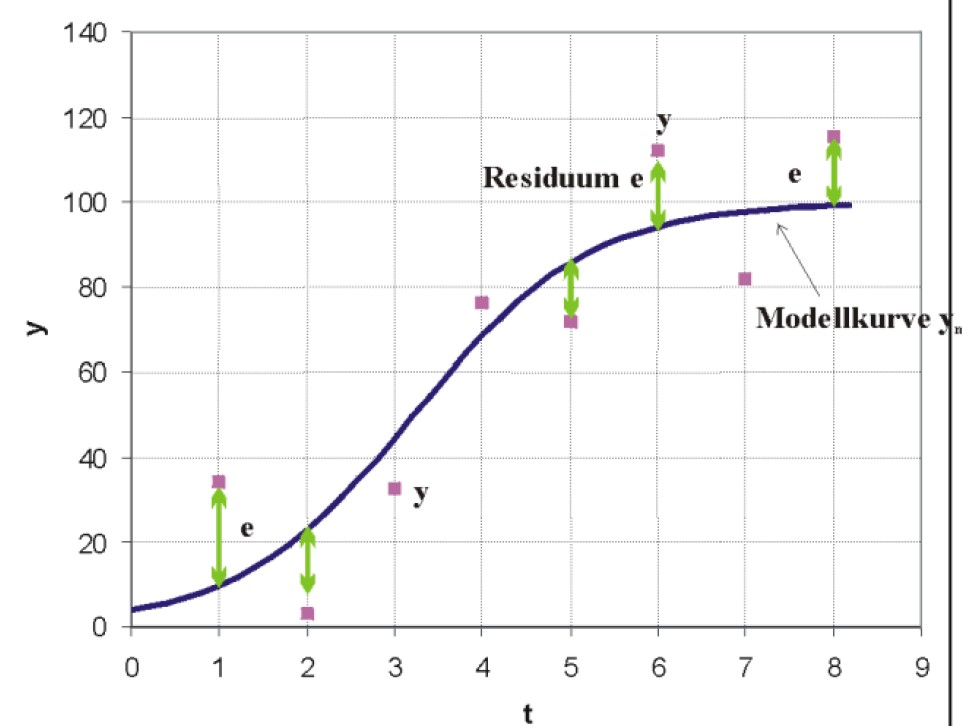
\includegraphics[width=0.45\textwidth]{images/Screenshot 2022-10-26 091954.jpg}
  \caption{Data approximated by an error curve}
  \label{fig:overview}
\end{wrapfigure}\newline
The approximation function can be described with a set of basis functions, which we name here $g_0, g_1, \ldots, g_m=\left\{g_j\right\}_{j=0, \ldots, m}$. Note the basis functions are sometimes also called  monomials.
Furthermore we define the following
\begin{itemize}
    \item N: Number of sample points
    \item m: degree of basic functions (m $\ll$ N)
    \item a: weighting coefficients
    \item $\left(x_0, y_0\right),\left(x_1, y_1\right)_1, \ldots,\left(x_N, y_N\right)=\left\{\left(x_i, y_i\right)\right\}_{i=0, \ldots, N}$: measurement points
\end{itemize}
With those variables one can create a equation in matrix notation form, as can be seen in \autoref{eq:leas_square_design_matrix}:

\begin{equation}\label{eq:leas_square_design_matrix}
\overbrace{\left(\begin{array}{cccc}
g_{0}\left(x_{0}\right) & g_{1}\left(x_{0}\right) & \ldots & g_{m}\left(x_{0}\right) \\
\vdots & \vdots & \ddots & \vdots \\
\vdots & \vdots & \ddots & \vdots \\
g_{0}\left(x_{N}\right) & g_{1}\left(x_{N}\right) & \ldots & g_{m}\left(x_{N}\right)
\end{array}\right)}^{\text {Designmatrix } G} \cdot\left(\begin{array}{c}
a_{0} \\
\vdots \\
a_{m}
\end{array}\right)=\left(\begin{array}{c}
y_{0} \\
\vdots \\
\vdots \\
y_{N}
\end{array}\right) \Leftrightarrow \quad G \cdot a=y
\end{equation}
Since \autoref{eq:leas_square_design_matrix} is normally overdetermined (m$\ll$N) The error/residuals can be calculated with \autoref{eq:least_square} and the squared sum S of residuals with \autoref{eq:least_square_squared}. The goal is now to minimize S from \autoref{eq:least_square_squared}. This can be done with \autoref{eq:least_square_g}, which is not derived in this post (for more information, search after orthogonal projection).



\begin{equation}\label{eq:least_square}
r_i=y_i-\sum_{j=0}^m a_j g_j\left(x_i\right) \quad(i=0, \ldots, N)
\end{equation}
\begin{equation} \label{eq:least_square_squared}
\underbrace{S}_{\text{Error}}=\sum_{i=0}^N\left(y_i-\underbrace{\sum_{j=0}^m a_j g_j\left(x_i\right)}_{\text{Model}}\right)^2=\sum_{i=0}^N r_i^2 \Rightarrow \min !
\end{equation}
\subsubsection{Thinking hint}
Lets assume one has the following points: $\{1,1\},\{2,2\}$ and one wants to approximate those points by a polynomial of degree zero ($m=0$) $\Rightarrow g_0(x)=1$. Then one can write the term inside the square brackets as the following:
$$
\overbrace{\left[\begin{array}{c}
1 \\
2 \\
\end{array}\right]}^{y}-
\overbrace{\left[\begin{array}{c}
1\\
1
\end{array}\right]}^{\textbf{G}} \cdot
\overbrace{\left[\begin{array}{c}
a
\end{array}\right]}^{a}
$$
But as one can see one can not take the square of this term, therefore one has to multiply on both left sides with $\textbf{G}^T$ which has no effect on the end result, since one is only interested in the minimum.
$$
\overbrace{\left[\begin{array}{cc}
1 & 1\\
\end{array}\right]}^{\textbf{$G^T$}} \cdot
\overbrace{\left[\begin{array}{c}
1 \\
2 \\
\end{array}\right]}^{y}-
\overbrace{\left[\begin{array}{cc}
1 &1
\end{array}\right]}^{\textbf{$G^T$}} \cdot
\overbrace{\left[\begin{array}{c}
1\\
1
\end{array}\right]}^{\textbf{G}} \cdot
\overbrace{\left[\begin{array}{c}
a
\end{array}\right]}^{a}
$$
When one squares the term above and says that $\textbf{G}^T\cdot y$ and $\textbf{G}^T\cdot \textbf{G}$ belong to each other, (are not separable) and then takes furthermore the derivative, one gets the following result: $2\cdot \left(a\cdot (\textbf{G}^T\cdot \textbf{G})-(\textbf{G}^T\cdot y)  \right)\cdot (\textbf{G}^T\cdot \textbf{G})$. When one sets this term to zero since one is interested in the minimum and solves it after $a$ one gets the result from \autoref{eq:least_square_g}.
\subsubsection{Normal equations}
\begin{equation}\label{eq:least_square_g}
\underbrace{\boldsymbol{G}^{T} \boldsymbol{G}}_{\text {Normal matrix }} \cdot \boldsymbol{a}=\boldsymbol{G}^{T} \boldsymbol{y} \quad \Rightarrow \quad \boldsymbol{a}=\left(\boldsymbol{G}^{T} \boldsymbol{G}\right)^{-1} \boldsymbol{G}^{T} \boldsymbol{y}
\end{equation}
$$
\begin{aligned}
& \underbrace{\underbrace{\boldsymbol{G}^{T}}_{(m+1) \times(N+1)}}_{(m+1) \times(m+1)} \cdot \underbrace{\boldsymbol{G}}_{(N+1) \times(m+1)} \cdot \underbrace{\boldsymbol{a}}_{(m+1) \times 1}=\underbrace{\boldsymbol{G}^{T}}_{(m+1) \times 1} \cdot \underbrace{\boldsymbol{y}}_{(N+1) \times 1}
\end{aligned}
$$
\subsection{Singular-value decomposition (SVD)}
A \href{https://en.wikipedia.org/wiki/Singular_value_decomposition}{singular-value decomposition} is one of the most widely used matrix operations in applied linear algebra.
\subsubsection{Idea}
Every Matrix $\boldsymbol{G}$ with the dimensions $(N+1) \times(m+1)$ can be decomposed as the triple product $\boldsymbol{U} \boldsymbol{D} \boldsymbol{V}^{T}$ whereas $\boldsymbol{U}$ is an \href{https://en.wikipedia.org/wiki/Orthogonal_matrix}{orthogonal} (N +1) × (N +1) -matrix, $\boldsymbol{D}$ is a (N +1) × (m +1) diagonal matrix and $\boldsymbol{V}$ again is orthogonal with dimensions (m +1) × (m +1). When a matrix is orthogonal, the following applies: $Q^{\mathrm{T}} Q=Q Q^{\mathrm{T}}=I$ and $Q^{\mathrm{T}}=Q^{-1}$. Due to that nice property, \autoref{eq:leas_square_design_matrix} can be calculated according to \autoref{eq:singular_value_decomposition_2}.
\begin{equation}\label{eq:singular_value_decomposition}
\boldsymbol{G}=\boldsymbol{U} \boldsymbol{D} \boldsymbol{V}^{T}=\boldsymbol{U} \cdot\left[\begin{array}{cccc}
d_{00} & 0 & \ldots & 0 \\
0 & d_{11} & \ldots & 0 \\
\vdots & \vdots & \ddots & 0 \\
0 & \ldots & 0 & d_{m m} \\
0 & 0 & \ldots & 0 \\
\vdots & \vdots & \ddots & 0 \\
0 & 0 & \ldots & 0
\end{array}\right] \cdot \boldsymbol{V}^{T}
\end{equation}


$G a_|=y_|$ becomes $U D V^{T} a_|=y_|$. Which results in \autoref{eq:singular_value_decomposition_2}
\begin{equation}\label{eq:singular_value_decomposition_2}
a_|=V D^{-1} U^{T} \cdot y_|
\end{equation}
% \subsubsection{Exercise one}

% \paragraph{Design matrix G}
% G: $(N+1)\cdot(m+1)$


% \begin{equation}
% \begin{array}{l|l|l|l|l|l} 
% & g_0 & g_1 & g_2 & \cdots & g_m \\
% \hline 
% x_0 & g_0\left(x_0\right) & g_1\left(x_0\right) &&\\
% x_1 & g_0\left(x_1\right) & g_1\left(x_1\right) && \\
% x_2 & \vdots & \vdots &&&\\
% x_N & g_0\left(x_N\right) & g_1\left(x_N\right) &&
% \end{array}
% \end{equation}
% With \autoref{eq:least_square} we can crete the following matrix


\subsubsection{Uniform arguments and orthogonal polynomials}
With uniform arguments $x_{i}-x_{j}=(j-i) h$ for all  $i, j \rightarrow\left\{x_{0} \ldots x_{N}\right\}=\left\{x_{0}+t \cdot h\right\}_{t=0 \ldots N}$ and orthogonal polynomials $G G^{T}$ can be diagonalized and therefore the equation can be easier solved. An example can be found in \autoref{subsubsec:orthognal_example}

\begin{equation}\label{eq:orthogonal_polynomials}
    \begin{aligned}
    p_{k, N}(t)&=\sum_{i=0}^{k}(-1)^{i}\left(\begin{array}{c}
    k \\
    i
    \end{array}\right)\left(\begin{array}{c}
    k+i \\
    i
    \end{array}\right) \frac{t^{(i)}}{N^{(i)}}\\&=1+\sum_{i=1}^{k}(-1)^{i}\left(\begin{array}{c}
    k \\
    i
    \end{array}\right)\left(\begin{array}{c}
    k+i \\
    i
    \end{array}\right) \frac{t(t-1)(t-2) \ldots(t-i+1)}{N(N-1)(N-2) \ldots(N-i+1)} \quad(k=1, \ldots, N)
    \end{aligned}
\end{equation}


with $t=\frac{x-x_{0}}{h} \quad\left(\begin{array}{l}k \\ i\end{array}\right)=\frac{k !}{i !(k-i) !}=n C r(k, i)$

$p_{k, N}$ can now with $g_{k}$ be put in the design matrix and the product $G^{T} G$ will be a $(m+1) \times(m+1)$ Diagonal matrix. Afterwards $a$ can be calculated with the knows formula $G^{T} G a=G^{T} y$.

\subsubsection{Calculation of the first terms for orthogonal polynomials:}\label{subsubsec:calc_orthog}
From \autoref{eq:orthogonal_polynomials} one knows that $N^{(i)}$ and $t^{(i)}$ are the following:
\begin{equation}
N^{(i)}=\underbrace{\underbrace{(N-1)}_{N^0}(N-2)}_{N^1}(N-2) \cdots(N-i+1)
\end{equation}
\begin{equation}
t^{(i)}=\underbrace{\underbrace{(t-0)}_{t^1}(t-1)}_{t^1}(t-2) \cdots(t-i+1)
\end{equation}


$$
p_{0, 4}(t)=\sum_{i=0}^0(-1)^0\left(\begin{array}{c}
0 \\
0
\end{array}\right)\left(\begin{array}{c}
0+0 \\
0
\end{array}\right) \frac{1\textcolor{gray}{=t^{0}}}{1=\textcolor{gray}{4^0}} =\underline{\underline{1}}
$$

$$
\begin{aligned}
p_{1, 4}(t)&=\sum_{i=0}^1(-1)^i\left(\begin{array}{c}
1 \\
i
\end{array}\right)\left(\begin{array}{c}
1+i \\
i
\end{array}\right) \frac{t^{i}}{N^{i}} \\
&=(-1)^0\underbrace{\left(\begin{array}{c}
1 \\
0
\end{array}\right)}_{=1}\underbrace{\left(\begin{array}{c}
1+0 \\
0
\end{array}\right)}_{=1} \frac{1\textcolor{gray}{=t^{(0)}}}{1=\textcolor{gray}{4^0}}\\&+
(-1)^1\underbrace{\left(\begin{array}{c}
1 \\
1
\end{array}\right)}_{=1}\underbrace{\left(\begin{array}{c}
1+1 \\
1
\end{array}\right)}_{=2} \frac{t\textcolor{gray}{=t^{(1)}}}{4=\textcolor{gray}{4^1}}\\ &=\underline{\underline{1-\frac{t}{2}}}
\end{aligned}
$$

$$
\begin{aligned}
p_{2, 4}(t)&=\sum_{i=0}^2(-1)^i\left(\begin{array}{c}
2 \\
i
\end{array}\right)\left(\begin{array}{c}
2+i \\
i
\end{array}\right) \frac{t^{i}}{N^{i}} \\
&=(-1)^0\underbrace{\left(\begin{array}{c}
2 \\
0
\end{array}\right)}_{=1}\underbrace{\left(\begin{array}{c}
2+0 \\
0
\end{array}\right)}_{=1} \frac{1\textcolor{gray}{=t^{(0)}}}{1=\textcolor{gray}{4^0}}\\&+
(-1)^1\underbrace{\left(\begin{array}{c}
2 \\
1
\end{array}\right)}_{=2}\underbrace{\left(\begin{array}{c}
2+1 \\
1
\end{array}\right)}_{=3} \frac{t\textcolor{gray}{=t^{(1)}}}{4=\textcolor{gray}{4-0}}\\&+
(-1)^2\overbrace{\left(\begin{array}{c}
2 \\
2
\end{array}\right)}^{=\frac{2 !}{2 !(2-2) !}=1}\underbrace{\left(\begin{array}{c}
2+2 \\
2
\end{array}\right)}_{=\frac{4 !}{2 !(4-2) !}=6} \frac{t\cdot(t-1)\textcolor{gray}{=t^2-t}}{4 \cdot (4-1)=\textcolor{gray}{12}}\\ &=\underline{\underline{1-\frac{3}{2}\cdot t+\frac{1}{2}\cdot t^2-\frac{1}{2}\cdot t}}
\end{aligned}
$$












% \subsubsection{Example:}

% $$
% \boldsymbol{x}=\left[\begin{array}{lllll}
% 3 & 4 & 5 & 6 & 7
% \end{array}\right] \quad \Rightarrow \quad \boldsymbol{t}=\boldsymbol{x}-3=\left[\begin{array}{lllll}
% 0 & 1 & 2 & 3 & 4
% \end{array}\right]
% $$

% $\Rightarrow P_{0}(x)=1 \quad P_{1}(x)=1-\frac{x-3}{2} \quad P_{2}(x)=1-\frac{2 \cdot 3(x-3)}{4}+\frac{1 \cdot 3(x-3)(x-3-1)}{4 \cdot 3}=1-\frac{3 x-9}{2}+\frac{1}{2}(x-4)(x-3) ? ? ?$

% $$
% \boldsymbol{G}=\left[\begin{array}{ccc}
% P_{0} & P_{1} & P_{2} \\
% 1 & 1 & 1 \\
% 1 & 1 / 2 & -1 / 2 \\
% 1 & 0 & -1 \\
% 1 & -1 / 2 & -1 / 2 \\
% 1 & -1 & 1
% \end{array}\right] \quad \Rightarrow \quad \boldsymbol{G}^{T} \boldsymbol{G}=\left[\begin{array}{ccc}
% \left\|P_{0}\right\|^{2} & 0 & 0 \\
% 0 & \left\|P_{1}\right\|^{2} & 0 \\
% 0 & 0 & \left\|P_{2}\right\|^{2}
% \end{array}\right]=\left[\begin{array}{ccc}
% 5 & 0 & 0 \\
% 0 & \frac{5}{2} & 0 \\
% 0 & 0 & \frac{7}{2}
% \end{array}\right]
% $$


\subsubsection{Exercise one, least square parabola}\label{subsubsec:least_square_ex1}
Compute a linear least-squares approximating parabola for the "second window" of five consecutive points (starting with x = 2) in the data.
$$
\begin{aligned}
\{\{x, y\}\}=&\{\{1,1.04\},\{2,1.37\},\{3,1.70\},\{4,2.00\},\{5,2.26\}\\
&\{6,2.42\},\{7,2.70\},\{8,2.78\},\{9,3.00\},\{10,3.14\}\}
\end{aligned}
$$
Lets also say the following:
\begin{itemize}
    \item m = deg = 2 (polys)  $\{1;x;x^2\}$
    \item N=4 (number of arguments actually 5 points)
\end{itemize}
Note: Normally: m$\ll$N (The degree is smaller than the number of points)
\paragraph{Write down the design matrix and the system of normal equations.}
$$
G=
\left\{\begin{array}{c|ccc}
 & g_0 & g_1 & g_2 \\
\hline 
x_0 & g_0\left(x_0\right) & g_1\left(x_0\right) & g_2\left(x_0\right) \\
x_1 & g_0\left(x_1\right) & g_1\left(x_1\right) & g_2\left(x_1\right)\\
x_2 &\vdots&\vdots&\vdots \\
x_3 &  \\
x_4 &  
\end{array}\right\}
=
\left\{\begin{array}{c|ccc}
 & 1 & x & x^2 \\
\hline 
2 & 1 & 2 & 4 \\
3 & 1 & 3 & 9 \\
4 & 1 & 4 & 16 \\
5 & 1 & 5 & 25 \\
6 & 1 & 6 & 36 
\end{array}\right\}
$$
\begin{equation}
\overbrace{\left(\begin{array}{ccc}
1 & 2 & 4 \\
1 & 3 & 9 \\
1 & 4 & 16 \\
1 & 5 & 25 \\
1 & 6 & 36 
\end{array}\right)}^{\text{Design matrix G}} \cdot\left(\begin{array}{l}
a_0 \\
a_1 \\
a_2
\end{array}\right)=\left(\begin{array}{l}
1.37 \\
1.70 \\
2.00 \\
2.26 \\
2.42 
\end{array}\right)
\end{equation}
With  \autoref{eq:least_square_g} we get the system of normal equations as one can see in \autoref{eq:least_squre_system_of_normal_equations}:
$$
\overbrace{\left[\begin{array}{ccccc}
1 & 1 & 1 & 1 & 1 \\
2 & 3 & 4 & 5 & 6 \\
4 & 9 & 16 & 25 & 36
\end{array}\right]}^{\textbf{G}^T} \cdot \overbrace{\left[\begin{array}{c}
1.37 \\
1.7 \\
2 \\
2.26 \\
2.42
\end{array}\right]}^{y} =\left[\begin{array}{c}
9.75 \\
41.66 \\
196.4
\end{array}\right]
$$
$$
\overbrace{\left[\begin{array}{ccccc}
1 & 1 & 1 & 1 & 1 \\
2 & 3 & 4 & 5 & 6 \\
4 & 9 & 16 & 25 & 36
\end{array}\right]}^{G^{T}G} \cdot \overbrace{\left[\begin{array}{ccc}
1 & 2 & 4 \\
1 & 3 & 9 \\
1 & 4 & 16 \\
1 & 5 & 25 \\
1 & 6 & 36
\end{array}\right]}^G=
\left[\begin{array}{ccc}
5 & 20 & 90 \\
20 & 90 & 440 \\
90 & 440 & 2274
\end{array}\right]
$$
\begin{equation}\label{eq:least_squre_system_of_normal_equations}
\overbrace{\left(\begin{array}{ccc}
5 & 20 & 90 \\
20 & 90 & 440 \\
90 & 440 & 2274
\end{array}\right)}^{G^{T}G} \cdot\left(\begin{array}{l}
a_0 \\
a_1 \\
a_2
\end{array}\right)=\left(\begin{array}{c}
9.75 \\
41.66 \\
196.4
\end{array}\right)
\end{equation}
\paragraph{Solve the linear system}
$$
\begin{aligned}
&a_0=0.506 ; a_1=0.483143 ; a_2=-0.0271429 \\
&y=a_0 \cdot 1+a_1 \cdot x+a_2\cdot x^2
\end{aligned}
$$
When one wants to increase the stability of the matrix one can make a statistical normalization.
\paragraph{Compute the output y and the derivative (!) of the approximation at the central coordinate (x = 4)} \label{par:result1}
$$
y(4)=\underline{\underline{2.00429}} ; \quad y^{\prime}(4)=a_1+2 a_2 \cdot 4=\underline{\underline{0.266}}
$$
\subsubsection{Excercise three, Savitzky Golay filter}
Apply the filter formulas developed in the exercise before for the data to compute approximately y for $x = 3, \dots , 8$
$$
\begin{array}{|l|cccccccccc|}
\hline \boldsymbol{x}_{\boldsymbol{k}} & \mathbf{1} & \mathbf{2} & \mathbf{3} & \mathbf{4} & \mathbf{5} & \mathbf{6} & \mathbf{7} & \mathbf{8} & \mathbf{9} & \mathbf{1 0} \\
\hline y_k & 1.04 & 1.37 & 1.70 & 2.00 & 2.26 & 2.42 & 2.70 & 2.78 & 3.00 & 3.14 \\
\hline
\end{array}
$$

$$
\begin{aligned}
&k=2 \Rightarrow x=3: a_0=y_2-\frac{3}{35} \Delta^4 y_0=1.7 c-\frac{3}{35} 0.02=1.6983 \\
&k=3 \Rightarrow x=4: a_0=y_3-\frac{3}{35} \Delta^4 y_1=2-\frac{3}{35}(-0.05)=2.0043 \\
&k=4 \Rightarrow x=5: a_0=y_4-\frac{3}{35} \Delta^4 y_2=2.26-\frac{3}{35}(0.28)=2.236 \\
&k=5 \Rightarrow x=6: a_0=y_5-\frac{3}{35} \Delta^4 y_3=2.42-\frac{3}{35}(-0.54)=2.4663 \\
&k=6 \Rightarrow x=7: a_0=y_6-\frac{3}{35} \Delta^4 y_4=2.7-\frac{3}{35}(0.66)=2.6434 \\
&k=7 \Rightarrow x=8: a_0=y_7-\frac{3}{35} \Delta^4 y_5=2.78-\frac{3}{35}(-0.56)=2.828
\end{aligned}
$$
\subsubsection{Exercise four, orthogonal polynomials}\label{subsubsec:orthognal_example}
Solve \autoref{subsubsec:least_square_ex1} again by using the orthogonal polynomials $\left\{p_{k, N}(t)\right\}_{k=0, \ldots, 2}$\newline
From \autoref{eq:orthogonal_polynomials} and \autoref{subsubsec:calc_orthog} one knows the three basis functions:
$$
P_{0,4}(t)=1=g_0 ; \quad P_{1,4}(t)=1-\frac{1}{2}t=g_1(t) ; \quad P_{2,4}(t)=1-2\cdot t +\frac{1}{2}t^2=g_2(t)
$$
Now we fist have to find a transformation. The transformation can be written in  the follwoing way:
$$
t=\frac{x-2}{1}=x-2 \in\{0, \cdots, 4\}
$$
$$
G=
\left\{\begin{array}{c|ccc}
 & g_0 & g_1 & g_2 \\
\hline 
t_0 & g_0\left(t_0\right) & g_1\left(t_0\right) & g_2\left(t_0\right) \\
t_1 & g_0\left(t_1\right) & g_1\left(t_1\right) & g_2\left(t_1\right)\\
t_2 &\vdots&\vdots&\vdots \\
t_3 &  \\
t_4 &  
\end{array}\right\}
=
\left\{\begin{array}{c|ccc}
 & 1 & 1-\frac{1}{2}t & 1-2\cdot t +\frac{1}{2}t^2 \\
\hline 
0 & 1 & 1 & 1 \\
1 & 1 & \frac{1}{2} & -\frac{1}{2} \\
2 & 1 & 0 & -1 \\
3 & 1 & -\frac{1}{2} & -\frac{1}{2} \\
4 & 1 & -1 & 1 
\end{array}\right\}
$$
\begin{equation}
\overbrace{\left(\begin{array}{ccc}
1 & 1 & 1 \\
1 & \frac{1}{2} & -\frac{1}{2} \\
1 & 0 & -1 \\
1 & -\frac{1}{2} & -\frac{1}{2} \\
1 & -1 & 1 
\end{array}\right)}^{\text{Design matrix G}} \cdot\left(\begin{array}{l}
a_0 \\
a_1 \\
a_2
\end{array}\right)=\left(\begin{array}{l}
1.37 \\
1.70 \\
2.00 \\
2.26 \\
2.42 
\end{array}\right)
\end{equation}
With  \autoref{eq:least_square_g} we get the system of normal equations as one can see in \autoref{eq:least_squre_system_of_normal_equations_ex4}:
$$
\overbrace{\left[\begin{array}{ccccc}
1 & 1 & 1 & 1 & 1 \\
1 & \frac{1}{2} & 0 & -\frac{1}{2} & -1 \\
1 & -\frac{1}{2} & -1 & -\frac{1}{2} & 1
\end{array}\right]}^{\textbf{G}^T} \cdot \overbrace{\left[\begin{array}{c}
1.37 \\
1.7 \\
2 \\
2.26 \\
2.42
\end{array}\right]}^{y} =\left[\begin{array}{c}
9.75 \\
-1.33 \\
-0.19
\end{array}\right]
$$
$$
\overbrace{\left[\begin{array}{ccccc}
1 & 1 & 1 & 1 & 1 \\
1 & \frac{1}{2} & 0 & -\frac{1}{2} & -1 \\
1 & -\frac{1}{2} & -1 & -\frac{1}{2} & 1
\end{array}\right]}^{G^{T}G} \cdot \overbrace{\left[\begin{array}{ccc}
1 & 1 & 1 \\
1 & \frac{1}{2} & -\frac{1}{2} \\
1 & 0 & -1 \\
1 & -\frac{1}{2} & -\frac{1}{2} \\
1 & -1 & 1 
\end{array}\right]}^G=
\left[\begin{array}{ccc}
5 & 0 & 0 \\
0 & \frac{5}{2} & 0 \\
0 & 0 & \frac{7}{2}
\end{array}\right]
$$
\begin{equation}\label{eq:least_squre_system_of_normal_equations_ex4}
\overbrace{\left(\begin{array}{ccc}
5 & 0 & 0 \\
0 & \frac{5}{2} & 0 \\
0 & 0 & \frac{7}{2}
\end{array}\right)}^{G^{T}G} \cdot\left(\begin{array}{l}
a_0 \\
a_1 \\
a_2
\end{array}\right)=\overbrace{\left(\begin{array}{c}
9.75 \\
-1.33 \\
-0.19
\end{array}\right)}^{y}
\end{equation}
When we now calculate $(G^{T}G)^{-1}\cdot y$ one gets $\left(\begin{array}{c}
1.95 \\
-0.532 \\
-\frac{0.38}{7}
\end{array}\right)$
The result is therefore:
$$
\begin{aligned}
&y(x)=a_0 \cdot 1+a_1 \cdot p_{1,4}(t)+a_2 \cdot p_{2,4}(x)\\
&y(x=4)=y(t=2)=a_0+a_1 \cdot 0+a_2(-1)=\underline{\underline{2,00429}}\\
&\begin{aligned}
y^{\prime}(x=4)&=\frac{1}{1} y^{\prime}(x=2)=a_1 p_{1,4}^{\prime}(2)+a_2 p_{2,4}^{\prime}(2).\\
&=a_1\left(-\frac{1}{2}\right)+\left(-2+2\right)=\underline{\underline{0.266}}
\end{aligned}
\end{aligned}
$$
Which is the same as in\autoref{par:result1}.







\subsubsection{Exercise five, singular value decomposition}
Examine and compute a least-squares approximative quadratic parabola for the data
$$
\begin{array}{|l|l|l|l|l|l|}
\hline x & -2 & -1 & 0 & 1 & 2 \\
\hline y & 0 & 1 & 2 & 3 & 1 \\
\hline
\end{array}
$$
with respect to the basis functions $\left\{1,-\frac{x}{2}, \frac{x^2}{2}-1\right\}$ in the following sense:
\paragraph{Compute the design matrix G and the normal matrix. Hint: The normal matrix here is diagonal!}
$$
G=
\left\{\begin{array}{c|ccc}
 & g_0 & g_1 & g_2 \\
\hline 
x_0 & g_0\left(x_0\right) & g_1\left(x_0\right) & g_2\left(x_0\right) \\
x_1 & g_0\left(x_1\right) & g_1\left(x_1\right) & g_2\left(x_1\right)\\
x_2 &\vdots&\vdots&\vdots \\
x_3 &  \\
x_4 &  
\end{array}\right\}
=
\left\{\begin{array}{c|ccc}
 & 1 & -\frac{x}{2} & \frac{x^2}{2}-1 \\
\hline 
-2 & 1 & 1 & 1 \\
-1 & 1 & \frac{1}{2} & -\frac{1}{2} \\
0 & 1 & 0 & -1 \\
1 & 1 & -\frac{1}{2} & -\frac{1}{2} \\
2 & 1 & -1 & 1 
\end{array}\right\}
$$

\begin{equation}
\overbrace{\left(\begin{array}{ccc}
1 & 1 & 1 \\
1 & \frac{1}{2} & -\frac{1}{2} \\
1 & 0 & -1 \\
1 & -\frac{1}{2} & -\frac{1}{2} \\
1 & -1 & 1 
\end{array}\right)}^{\text{Design matrix G}} \cdot\left(\begin{array}{l}
a_0 \\
a_1 \\
a_2
\end{array}\right)=\left(\begin{array}{l}
0 \\
1 \\
2 \\
3 \\
1 
\end{array}\right)
\end{equation}
$$
\overbrace{\left[\begin{array}{ccccc}
1 & 1 & 1 & 1 & 1 \\
1 & \frac{1}{2} & 0 & -\frac{1}{2} & -1 \\
1 & -\frac{1}{2} & -1 & -\frac{1}{2} & 1
\end{array}\right]}^{\textbf{G}^T} \cdot \overbrace{\left[\begin{array}{c}
0 \\
1 \\
2 \\
3 \\
1 
\end{array}\right]}^{y} =\left[\begin{array}{c}
7 \\
-2 \\
-3
\end{array}\right]
$$
$$
\overbrace{\left[\begin{array}{ccccc}
1 & 1 & 1 & 1 & 1 \\
1 & \frac{1}{2} & 0 & -\frac{1}{2} & -1 \\
1 & -\frac{1}{2} & -1 & -\frac{1}{2} & 1
\end{array}\right]}^{G^{T}G} \cdot \overbrace{\left[\begin{array}{ccc}
1 & 1 & 1 \\
1 & \frac{1}{2} & -\frac{1}{2} \\
1 & 0 & -1 \\
1 & -\frac{1}{2} & -\frac{1}{2} \\
1 & -1 & 1 
\end{array}\right]}^G=
\left[\begin{array}{ccc}
5 & 0 & 0 \\
0 & \frac{5}{2} & 0 \\
0 & 0 & \frac{7}{2}
\end{array}\right]
$$
\begin{equation}\label{eq:least_squre_system_of_normal_equations_ex5}
\overbrace{\left(\begin{array}{ccc}
5 & 0 & 0 \\
0 & \frac{5}{2} & 0 \\
0 & 0 & \frac{7}{2}
\end{array}\right)}^{G^{T}G} \cdot\left(\begin{array}{l}
a_0 \\
a_1 \\
a_2
\end{array}\right)=\overbrace{\left(\begin{array}{c}
7 \\
-2 \\
-3
\end{array}\right)}^{y}
\end{equation}


\paragraph{Solve the system of normal equations and write down a formula for the approximating parabola.}
$$
\left[
\begin{array}{ccc|ccc}
5 & 0 & 0  & 1 & 0 & 0 \\
0 & \frac{5}{2} & 0  & 0 & 1 & 0 \\
0 & 0 & \frac{7}{2} & 0 & 0 & 1 \\
\end{array}
\right]
$$
divide first row by factor 5.
$$
\left[
\begin{array}{ccc|ccc}
1 & 0 & 0  & \frac{1}{5} & 0 & 0 \\
0 & \frac{5}{2} & 0  & 0 & 1 & 0 \\
0 & 0 & \frac{7}{2} & 0 & 0 & 1 \\
\end{array}
\right]
$$
Also divide other rows by its factor.
$$
\left[
\begin{array}{ccc|ccc}
1 & 0 & 0  & \frac{1}{5} & 0 & 0 \\
0 & 1 & 0  & 0 & \frac{2}{5} & 0 \\
0 & 0 & 1  & 0 & 0 & \frac{2}{7} \\
\end{array}
\right]
$$

$$
\overbrace{\left(\begin{array}{ccc}
\frac{1}{5} & 0 & 0 \\
0 & \frac{2}{5} & 0 \\
0 & 0 & \frac{2}{7}
\end{array}\right)}^{(G^{T}G)^{-1}} \cdot\overbrace{\left(\begin{array}{l}
7 \\
-2 \\
-3

\end{array}\right)}^{y}=\left(\begin{array}{c}
a_0 \\
a_1 \\
a_2
\end{array}\right)
$$


$$
\begin{aligned}
&a_0=\frac{7}{5}, a_1=-\frac{4}{5}, a_2=-\frac{6}{7} \\
&y=a_0 \cdot 1+a_1 \cdot -\frac{x}{2}+a_2 \frac{x^2}{2}-1\\
&y=\frac{7}{5} \cdot 1+-\frac{4}{5} \cdot -\frac{x}{2}+-\frac{6}{7} (\frac{x^2}{2}-1)\\
&y=\frac{7}{5}+\frac{2}{5} \cdot x+\frac{6}{7}-\frac{3}{7}\cdot x^2\\
&y=\frac{79}{35}+\frac{2}{5} \cdot x-\frac{3}{7}\cdot x^2
\end{aligned}
$$
\paragraph{What are the dimensions of the unitary matrices $U, V$ , as well as the diagonal matrix $D$, in the singular value decomposition $G = U D V^{tr}$}
\begin{itemize}
    \item U=5x5
    \item D=5x3
    \item V=3x3
\end{itemize}
\paragraph{What are the entries (singular values) in the matrix D from above}
The singular values are the square-root of the non zero eigenvalues of $\textbf{G}^T\cdot \textbf{G}$ and therefore $\{\sqrt{5} ; \sqrt{5 / 2} ; \sqrt{7 / 2}\}$
\paragraph{Give three orthogonal basis polynomials (with respect to the data given) as formulas in the variable x.}
$\left\{1 ;-\frac{x}{2} ; \frac{x^2}{2}-1\right\}$ is orthogonal because $\textbf{G}^T\cdot \textbf{G}$  is diagonal.







\subsection{Chebyshev polynomials}
\subsubsection{Idea}
Approximate a continuous polynomial by a Chebyshev polynomial. 
\subsubsection{Definition}
Chebyshev Polynomials are defined as $T_{n}(x)=\cos (n \arccos (x))$ with $(n=0,1, \ldots)$ and $(-1 \leq x \leq 1)$. Due to that, most data points are at the edge. The first polynomials can be found in \autoref{eq:chebychef_polynomials}.

\begin{equation} \label{eq:chebychef_polynomials}
\begin{aligned}
T_{0} & =1 && x^{0}=1=T_{0} \\
T_{1} & =x && x^{1}=x=T_{1} \\
T_{2} & =2 x^{2}-1 && x^{2}=\frac{1}{2} T_{2}+\frac{1}{2} T_{0} \\
T_{3} & =4 x^{3}-3 x && x^{3}=\frac{1}{4} T_{3}+\frac{3}{4} T_{1} \\
T_{4} & =8 x^{4}-8 x^{2}+1 && x^{4}=\frac{1}{8} T_{4}+\frac{1}{2} T_{2}+\frac{3}{8} T_{0} \\
T_{5} & =16 x^{5}-20 x^{3}+5 x && x^{5}=\frac{1}{16} T_{5}+\frac{5}{16} T_{3}+\frac{5}{8} T_{1}
\end{aligned}
\end{equation}
Further polynomials can be calculated with the recursion formula $T_{n+1}(x)=2 x T_{n}(x)-T_{n-1}(n \geq 2)$ with the initial conditions  $T_{1}(x)=x, T_{0}(x)=1$.
\subsubsection{Properties}
\begin{itemize}
    \item The maximal amplitude of a  Chebyshev-Polynomials is $\frac{1}{2^{n}}$ and for a normalized one $\frac{1}{2^n} T_{n+1}(x)$
    \item Amplitude: $T_{n}(x) \in[-1,+1]$
    \item Zero points: $T_{n}(x)=0 \Leftrightarrow x=\cos \left(\frac{2 i+1}{2 n} \pi\right) \quad i=0,1, \ldots, n-1$ (also called chebyshev knots)
    \item $T_{n}(x)=\pm 1 \Leftrightarrow x=\cos \left(\frac{i \pi}{n}\right)(i=0,1, \ldots, n)$
\end{itemize}


\subsubsection{Usage}
For Chebychev we use not $g$ but $T_x$ as function.
$$
G=\overbrace{
\left\{\begin{array}{c|ccccc}
 & T_0(x) & T_1(x) & T_2(x) &\cdots&T_m(x)\\
\hline 
x_0 & 1 & x_0 & 2\cdot x_0^2-1 \\
x_1 & 1 & x_1 & 2\cdot x_1^2-1 \\
x_2 & 1 & x_2 & 2\cdot x_2^2-1 \\
x_3 &  \vdots&\vdots&\vdots \\
x_N &  1 & x_N & 2\cdot x_N^2-1
\end{array}\right\}}^{Design Matrix}
=\left[\begin{array}{cccc}T_{0}\left(x_{0}\right)=1 & T_{1}\left(x_{0}\right)=x_{0} & \ldots & T_{m}\left(x_{0}\right) \\
T_{0}\left(x_{1}\right)=1 & T_{1}\left(x_{1}\right)=x_{1} & \ldots & T_{m}\left(x_{1}\right) \\
\vdots & \vdots & \ddots & \vdots \\
T_{0}\left(x_{N}\right)=1 & T_{1}\left(x_{N}\right)=x_{N} & \ldots & T_{m}\left(x_{N}\right)
\end{array}\right]_{N \times m}
$$
The matrix $G^{T}G$ can be callculated accroding to \autoref{eq:least_square_chebychef}.
\begin{equation}\label{eq:least_square_chebychef}
\begin{aligned}
&\left\langle T_j, T_k\right\rangle:=\sum_{i=0}^N T_j\left(x_i\right) T_k\left(x_i\right)=\left\{\begin{array}{cc}
0 & j \neq k \\
(N+1) / 2 & j=k \neq 0 \\
N+1 & j=k=0
\end{array} \quad(j, k=0, \ldots, N)\right. \\
&x_i=\cos \left(\frac{2 i+1}{2(N+1)} \pi\right) \quad(i=0,1, \ldots, N)
\end{aligned}
\end{equation}
And results then in the follwing matrix
$$
G^{T} G \underbrace{=}_{\text {When Chebyshev }}\left[\begin{array}{cccc}
N+1 & 0 & \cdots & 0 \\
0 & \frac{N+1}{2} & \cdots & 0 \\
\vdots & \vdots & \ddots & \vdots \\
0 & 0 & \ldots & \frac{N+1}{2}
\end{array}\right]_{m \times m}
$$
$$
\left(G^{T} G\right)^{-1} G^{T} \underbrace{=}_{\text {When Chebyshev }}\left[\begin{array}{cccc}
\frac{1}{N+1} T_{0}\left(x_{0}\right)=\frac{1}{N+1} & \frac{1}{N+1} T_{0}\left(x_{1}\right)=\frac{1}{N+1} & \cdots & \frac{1}{N+1} T_{0}\left(x_{N}\right)=\frac{1}{N+1} \\
\frac{2}{N+1} T_{1}\left(x_{0}\right)=\frac{2}{N+1} x_{0} & \frac{2}{N+1} T_{1}\left(x_{1}\right)=\frac{2}{N+1} x_{1} & \cdots & \frac{2}{N+1} T_{1}\left(x_{N}\right)=\frac{2}{N+1} x_{N} \\
\vdots & \vdots & \ddots & \vdots \\
\frac{2}{N+1} T_{m}\left(x_{0}\right) & \frac{2}{N+1} T_{m}\left(x_{1}\right) & \cdots & \frac{2}{N+1} T_{m}\left(x_{N}\right)
\end{array}\right]_{m \times N}
$$

\begin{multicols}{2}
[]
\paragraph{Recipe}
Goal: $y(t)=p_{N}(t)$ (define polynomial in $[a, b]$ ) with  Chebyshev-polynomials of degree $m$.
 \begin{enumerate}
    \item transform $y(t)$ on the standard interval $[-1,1]$ (affine Transformation) $t=a+\frac{b-a}{2}(x+1)$.
    \item describe $y(x)$ with $T_{n}$ terms
    \item truncate $y(x)$ on degree $m$ : $y_{m}(x)$
    \item back transformation: $x=2 \frac{t-a}{b-a}-1$
    \item insert $T_{n}$ in $y_{m}$ see \autoref{eq:chebychef_polynomials}
    \item error estimation for truncate Method:  \newline $\max _{t}\left|y(t)-y_{m}(t)\right|($ removed part$)$
 \end{enumerate}\mbox{}\newline{}\newline
 \paragraph{Example}
 Approximation of $y(t)=t^{3}$ with degree $m=2$ for the interval $(a, b)=(0,1)$
 \begin{enumerate}
    \item Transformation with $t=\frac{x+1}{2}$ 
    $$
    y(x)=\left(\frac{x+1}{2}\right)^{3}=\frac{1}{8}\left(x^{3}+3 x^{2}+3 x+1\right)
    $$
    \item Expand with $T_{n}$ see also \autoref{eq:chebychef_polynomials}:
    $$
    \begin{aligned}
    & y(x)=\frac{1}{8}\left(\frac{T_{3}(x)+3 T_{1}(x)}{4}+3 \frac{T_{2}(x)+T_{0}}{2}+3 T_{1}(x)+T_{0}(x)\right) \\
    & =\frac{1}{32} T_{3}(x)+\frac{3}{16} T_{2}(x)+\frac{15}{32} T_{1}(x)+\frac{5}{16} T_{0}(x)
    \end{aligned}
    $$
    \item shorten to degree $m=2$ :
     $y(x) \approx \frac{3}{16} T_{2}(x)+\frac{15}{32} T_{1}(x)+\frac{5}{16} T_{0}(x)$
    \item back transformation with $x=2 t-1$ :
     $y(t) \approx \frac{3}{16} T_{2}(2 t-1)+\frac{15}{32} T_{1}(2 t-1)+\frac{5}{16} T_{0}(2 t-1)$
    \item $T_{n}(2 t-1)$ substitution:
     $y(t) \approx \frac{3}{16}\left(2(2 t-1)^{2}-1\right)+\frac{15}{32}(2 t-1)+\frac{5}{16}$
    \item error estimation:
     $\max _{t}\left|\frac{1}{32} T_{3}(2 t-1)\right|$ 
 \end{enumerate}
\end{multicols}





\subsection{Continuous Chebyshev approximation}
A weight function $w(x)$ is often called the function inside the integral, in the case of the formula below $w(x)=\frac{1}{\sqrt{1-x^2}}$.
\begin{equation}\label{eq:continuous_inner_product}
\left\langle T_j, T_k\right\rangle_{\text {cont }}:=\int_{-1}^1 T_j(x) T_k(x) \frac{d x}{\sqrt{1-x^2}}=\left\{\begin{array}{cc}
0 & j \neq k \\
\pi / 2 & j=k \neq 0 \\
\pi & j=k=0
\end{array}\right.
\end{equation}
\autoref{eq:continuous_inner_product} is true because the polynomial is orthogonal!
\paragraph{Example:Chebyshev continuous least-squares parabola on the interval $[0,1]$ for $y(t)=t^3$
First the interval $[0,1]$ is transformed to $[-1,1]$ by $x=2t-1$}
This is shown with \autoref{eq:transform_to_normal}
$$
-1+2 \frac{x-a}{b-a}=-1+2 \frac{x-0}{1-0}=1-2x
$$
In our case our new x is called t. Therefore $x=2t-1 \Rightarrow t=\frac{x+1}{2} \Rightarrow y(t)=\frac{(x+1)^3}{8}$
Now we can use \autoref{eq:continuous_formula} and get the following results:
$$
\begin{aligned}
&a_0=\frac{1}{\pi} \int_{-1}^1 y(x) \frac{d x}{\sqrt{1-x^2}}=\frac{5}{16}\\
&a_1=\frac{2}{\pi} \int_{-1}^1 y(x) T_1(x) \frac{d x}{\sqrt{1-x^2}}=\frac{15}{32}\\
&a_2=\frac{2}{\pi} \int_{-1}^1 y(x) T_2(x) \frac{d x}{\sqrt{1-x^2}}=\frac{3}{16}\\
\end{aligned}
$$

\begin{equation}\label{eq:continuous_formula}
p(x)=\sum_{j=0}^{m} a_{j} T_{j}(x) \quad \text { wobei } \quad a_{j}= \begin{cases}\frac{1}{\pi} \int_{-1}^{1} \frac{y(x)}{\sqrt{1-x^{2}}} d x & j=0 \\ \frac{2}{\pi} \int_{-1}^{1} \frac{y(x) T_{j}(x)}{\sqrt{1-x^{2}}} d x & j>0\end{cases}
\end{equation}
\subsection{Continuous Least-Square Legendre approximation}
\paragraph{Legendre Polynomials:}
The Legendre polynomials are defined by the Rodriguez formula which can be seen in \autoref{eq:Rodriguez}
\begin{equation}\label{eq:Rodriguez}
P_n(x)=\frac{1}{2^n n !} \cdot \frac{d^n}{d x^n}\left(x^2-1\right)^n
\end{equation}
Where the first polynomials can be seen in \autoref{eq:legendre_polynomials_first_view_examples}
\begin{equation}\label{eq:legendre_polynomials_first_view_examples}
    \begin{aligned}
    & P_{n}(x)=\frac{1}{2^{n} n !} \cdot \frac{\mathrm{d}^{n}}{\mathrm{~d} x^{n}}\left(x^{2}-1\right)^{2} \quad P_{0}(x)=1 \quad P_{1}(x)=x \quad P_{2}(x)=\frac{1}{2}\left(3 x^{2}-1\right) \\
    & P_{3}(x)=\frac{1}{2}\left(5 x^{3}-3 x\right) \quad P_{4}(x)=\frac{1}{8}\left(35 x^{4}-30 x^{2}+3\right) \quad P_{5}(x)=\frac{1}{8}\left(63 x^{5}-70 x^{3}+15 x\right)
    \end{aligned}
\end{equation}

\paragraph{Continuous Legendre least-squares approximation}\mbox{}\newline
If $y(x)$ is function on $[-1,1]$ which is absolutely square-integrable with respect to the weight function $w(x)=1 \quad(x \in[-1,1])$ in the sense that $\int_{-1}^1|y(x)|^2 d x<\infty$, then the continuous square-sum of residuals in \autoref{eq:legendre_square_sum}
\begin{equation}\label{eq:legendre_square_sum}
S:=\int_{-1}^1\left(y(x)-\sum_{j=0}^m a_j P_j(x)\right)^2 d x
\end{equation}
Is minimal when the coefficients $a$ have the value given in \autoref{eq:legendre_a_coefficients}. This equation also describes the resulting polynomial.
\begin{equation}\label{eq:legendre_a_coefficients}
p(x)=\sum_{j=0}^{m} a_{j} P_{j}(x) \quad \text { whereas } \quad a_{j}=\frac{2 j+1}{2} \cdot \int_{-1}^{1} y(x) P_{j}(x) \cdot \mathrm{d} x \quad(j=0,1, \ldots, m)
\end{equation}
where m is the degree.
\subsubsection{Legendre continuous least square parabola}
Legendre continuous least-squares parabola on the interval $t \in[0,1]$ for $y(t)=t^3$.\newline\newline

First one has to do a \href{https://borea17.github.io/ML_101/probability_theory/remap-numbers-in-interval}{transformation} to the interval $x \in[-1,1]$. This results in the following: $x=2 t-1 \Rightarrow t=\frac{x+1}{2}$, therefore $y(x)=\frac{(x+1)^3}{8}$. With \autoref{eq:legendre_a_coefficients} one gets then the following:
$$
\begin{aligned}
& a_0=\frac{1}{2} \int_{-1}^1 \underbrace{y(x)}_{\frac{(x+1)^3}{8}} \underbrace{P_0(x)}_{1} d x=\frac{1}{2} \int_{-1}^1 y(x) d x=\frac{1}{4} \\
& a_1=\frac{3}{2} \int_{-1}^1 y(x) P_1(x) d x=\frac{3}{2} \int_{-1}^1 y(x) x d x=\frac{9}{20} \\
& a_2=\frac{5}{2} \int_{-1}^1 y(x) P_2(x) d x=\frac{5}{2} \int_{-1}^1 y(x)\left(\frac{3 x^2-1}{2}\right) d x=\frac{1}{4}
\end{aligned}
$$
\subsection{Mulit-variate least-square}
Note: the degree of a multi-variate polynomial can be identified by adding up the degrees of the variables in each of the terms. It does not matter that there are different variables. The largest number is the degree.
\begin{itemize}
    \item Input bi-variate (x,y) 2D : $\Vec{x}$
    \item Output scalar Z: 1D
\end{itemize}

\begin{itemize}
    \item Degree 3. 
    $$
    \left\{1, x, y, x^{2}, 2 x y, y^{2}, x^{3}, 3 x^{2} y, 3 x y^{2}, y^{3}\right\}
    $$
    \item Degree 4. 
    $$
    \left\{1, x, y, x^{2}, 2 x y, y^{2}, x^{3}, 3 x^{2} y, 3 x y^{2}, y^{3}, x^{4}, 4 x^{3} y, 6 x^{2} y^{2}, 4 x y^{3}, y^{4}\right\}
    $$
\end{itemize}
Residuals: $r_i=z_i-f(\Vec{x_i}) \Rightarrow \sum r_i^2 \rightarrow min!$
$$
G=
\overbrace{\left\{\begin{array}{c|ccc}
 & g_0 & g_1 & g_2 \\
\hline 
\vec{x_0} & g_0\left(x_0\right) & g_1\left(x_0\right) & g_2\left(x_0\right) \\
\vec{x_1} & g_0\left(x_1\right) & g_1\left(x_1\right) & g_2\left(x_1\right)\\
\vec{x_2} &\vdots&\vdots&\vdots \\
\vdots    &  \\
\vec{x_N} &  
\end{array}\right\}}^{\text{Design matrix}}=
\left\{\begin{array}{c|ccccc}
 & 1 & y & y^2 & \cdots & xy^2 \\
\hline 
\vec{x_0} & 1 & y_0 & y_0^2 &~&\vdots\\
\vec{x_1} & 1 & y_1 & y_1^2\\
\vec{x_2} &\vdots&\vdots&\vdots \\
\vdots    &  \\
\vec{x_N} & 1 & y_N & y_N^2
\end{array}\right\}
$$
\paragraph{Basis Functions}
d=dim=2
$$
\sum_{j_1=0}^{m_1} \sum_{j_2=0}^{m_2} \cdots \sum_{j_d=0}^{m_d} \textcolor{olive}{a_{j_1, j_2, \ldots, j_d}} \textcolor{red}{g_{j_1}\left(x^{(1)}\right) g_{j_2}\left(x^{(2)}\right) \cdots g_{j_d}\left(x^{(d)}\right)}
$$
\paragraph{Product}
$$
\underbrace{\left\{1, x\right\}}_{\text{'2'}}x\underbrace{\left\{1, y, y^2\right\}}_{\text{'3'}}
$$
$$
\left\{1, y, y^2,x,xy,xy^2 \right\}=\text{'6'}
$$
\paragraph{Statistical norm}
$$
\left\{\left(\frac{x^{(1)}-\mu_1}{\sigma_1}\right)^j\left(\frac{x^{(2)}-\mu_2}{\sigma_2}\right)^k \mid j, k \in N_0\right\}
$$
% \subsection{SVD (Singular value decomposition)}
% Singular value decomposition means that one can transform a matrix into three single operations (rotations, stretching, rotation).
% \begin{itemize}
%     \item D: diagonal
%     \item U: orthogonal (N+1)x(N+1)
%     \item V orthogonal (m+1)x(m+1)
% \end{itemize}
% $$
% G=U D V^{t r}=U \cdot\overbrace{\left(\begin{array}{cccc}
% d_{00} & 0 & \cdots & 0 \\
% 0 & d_{11} & \ddots & \vdots \\
% \vdots & \ddots & \ddots & 0 \\
% 0 & \cdots & 0 & d_{m m} \\
% - & - & - & - \\
% 0 & \cdots & \cdots & 0 \\
% \vdots & \ddots & \ddots & \vdots \\
% 0 & \cdots & \cdots & 0
% \end{array}\right)}^{D} \cdot V^{t r}
% $$
% $$
% U=G\cdot G^{tr}
% $$
% $$
% V=G^{tr}\cdot G 
% $$
% One can now derive the following, which makes the calculation much easier.
% $$
% \begin{array}{|cccccc|}
% \hline \hat{r}_0 & = & \hat{y}_0-d_{00} \hat{a}_0- & 0 & -\cdots- & 0 \\
% \hat{r}_1 & = & \hat{y}_1-0 & d_{11} \hat{a}_1 & -\cdots- & \vdots \\
% \vdots & \vdots & \vdots & \ddots & \ddots & 0 \\
% \hat{r}_m & = & \widehat{y}_m-0 & \cdots & 0 & d_{m m} \widehat{a}_m \\
% \widehat{r}_{m+1} & = & \hat{y}_{m+1}-0 & \cdots & \cdots & 0 \\
% \vdots & \vdots & \vdots & \ddots & \ddots & \vdots \\
% \hat{r}_N & = & \hat{y}_N-0 & \cdots & \cdots & 0 \\
% \hline
% \end{array}
% $$
\subsubsection{Example one}
Normally, a set of four 3d-points $(x, y, z)$ is not contained in one single plane. But generally there
is a plane coming close to the 3d-points in the sense of least-squares approximation.\newline
The $(x, y, z)$-data in this problem is: A = (1,0,0), B = (0,1,0), C = (0,2,-1), D = (1,3,1)
\begin{enumerate}[label=(\alph*)]
    \item Give a reasonable set of basis functions. Hint: A plane has total degree 1 (complete basis) \newline\newline
    As a basis function, one can use:
    $$
\left\{1,x,y\right\}
$$


    \item Write down the design matrix according to a) and the normal equations
$$
G=
\overbrace{\left\{\begin{array}{c|ccc}
 & g_0 & g_1 & g_2 \\
\hline 
\vec{x_0} & g_0\left(\vec{x_0}\right) & g_1\left(\vec{x_0}\right) & g_2\left(\vec{x_0}\right) \\
\vec{x_1} & g_0\left(\vec{x_1}\right) & g_1\left(\vec{x_1}\right) & g_2\left(\vec{x_1}\right)\\
\vec{x_2} &\vdots&\vdots&\vdots \\
\vdots   &  \\
\vec{x_N} &  
\end{array}\right\}}^{\text{Design matrix}}=
\left\{\begin{array}{c|ccc}
 & 1 & x & y\\
\hline 
(1,0) & 1 & 1 & 0\\
(0,1) & 1 & 0 & 1\\
(0,2) & 1 & 0 & 2\\
(1,3) & 1 & 1 & 3\\
\end{array}\right\}
$$
    \item Solve the system of normal equations and give a functional formula for the
approximating plane.\newline\newline
According to \autoref{eq:least_square_g} to following is true: $\underbrace{\vec{a}=\left(G^T\cdot G\right)^{-1}G^T\cdot y}_{\text{normal equations}}$
$$
\vec{a}=
\left[\begin{array}{ccc}
-\frac{4}{5} \\
1 \\
\frac{1}{5} 
\end{array}\right]
$$
$$
f(x,y)=-\frac{4}{5}+x+\frac{1}{5}y
$$
\end{enumerate}
\subsubsection{Example three} \label{subsub:Example_cheby}
Express $x^3,x^4$ as linear combinations of the Chebyshev polynomials $T_0(x), T_1(x), T_2(x), T_3(x), T_4(x)$. \newline\newline
From \autoref{eq:chebychef_polynomials} one knows that $T_3(x)=4 x^3-3 x \Rightarrow \frac{1}{4}T_3(x)=x^3-\frac{3}{4}x \Rightarrow \underline{\underline{\frac{1}{4}T_3(x)+\frac{3}{4}T_1(x)}}=x^3$\newline\newline\newline
From \autoref{eq:chebychef_polynomials} one knows that $T_4(x)=8 x^4-8 x^2+1 \Rightarrow \frac{1}{8}T_4(x)=x^4-x^2+\frac{1}{8} \Rightarrow \frac{1}{8}T_4(x)+\frac{1}{2}T_2(x)=x^4-\frac{3}{8}\Rightarrow \underline{\underline{\frac{1}{8}T_4(x)+\frac{1}{2}T_2(x)+\frac{3}{8}T_0}}=x^4$

\subsubsection{Example six}
Express $x^3$ as linear combinations of the Legendre polynomials $P_0(x), P_1(x), P_2(x), P_3(x)$. \newline
From \autoref{eq:legendre_polynomials_first_view_examples} one knows that $P_3(x)=\frac{1}{2}\left(5 x^3-3 x\right) \Rightarrow \frac{2}{5}P_3(x)=x^3-\frac{3}{5}x \Rightarrow \underline{\underline{\frac{2}{5}P_3(x)+\frac{3}{5}P_1(x)}}=x^3$
\subsubsection{Example seven}
Compute continuously approximating least-squares lines for the model function
$y(t)=t^2$ $(0\geq t \geq 1 )$ by
\begin{enumerate}[label=(\alph*)]
    \item Chebyshev approximation with the weight function $w(x)=1 / \sqrt{1-x^2} \quad(-1<x<1)$\newline\newline
    Firstly one has to bring it into the correct range. One can do that with \autoref{eq:transform_to_normal} \newline
    Map the interval [a,b] onto the interval [c,d] 
    \begin{equation}
f(t)=c+\left(\frac{d-c}{b-a}\right)(t-a)
\end{equation}
$$
\underbrace{f(t)}_{x}=-1+\left(\frac{1+1}{1-0}\right)(t-0)=-1+2t \Rightarrow x=-1+2t \Rightarrow t=\frac{1}{2}(x+1) 
$$
$$
y=\frac{1}{4} x^2+\frac{1}{2} x+\frac{1}{4}
$$
$$
y=\frac{1}{4} x^2+\frac{1}{2} x+\frac{1}{4}
$$
$$
\frac{1}{8}T_2=\frac{1}{4} x^2-\frac{1}{8}\Rightarrow \frac{1}{8}T_2+\frac{1}{2}T_1+\frac{3}{8}T_0\Rightarrow \underline{line=\frac{3}{8}+\frac{1}{2}x}=\underline{\underline{\frac{3}{8}+\frac{1}{2}(2t-1)}}
$$
\item Legendre approximation with the weight function $w(x)=1$
    \item Estimate the maximum approximating errors in ab) by the coefficients of the Chebyshev polynomial $T_2(x)$ and Legendre polynomial $P_2(x)$ , respectively
    
\end{enumerate}